\chapter{Background (18)}
\label{ch:background}

The aim of this chapter is to give the reader background information on the problem domain in order for them
to understand the rest of the report.
There will also be a in-depth discussion of existing literature that relates to machine learning in texas hold'em
agents.

Machine learning is an area of computer science that tackles how we construct computer programs that improve
with experience\citep{mitchell1997machine}.
The term was coined by Arthur Samuel in his 1959 paper where he discussed machine learning methods using
checkers.
Since then there has been a great deal of advancement in the field.
Some of the notable early contributions being the discovery of recurrent neural networks in 1982,
the advancement of reinforcement learning by the introduction of Q-Learning in 1989 and the
development of a backgammon-playing agent using neural networks and temporal difference learning\citep{tesauro1995td}.
Recently we have seen some of this early academic work culminate in more practical achievements such as
Facebook's DeepFace system which, in 2014,  was shown to be able to recognise faces at a rate of 97.35\% accuracy,
a rate that is comparable to that of humans.
Another example of recent achievement is Google's AlphaGo program which, in 2016, became the first program to beat
a professional human player.

It should be becoming clear that machine learning can be a solution to a wide array of problems and as
both hardware and software continue to improve it's reach will only continue to grow.
We are starting to see machine learning systems become a key component of many companies business model.
Since certain machine learning techniques are great at prediction, machine learning has been widely used
for content discovery by companies such as Google and Pinterest.
Other business applications include the use of chatbots as a part of customer service, self-driving cars
and even in the field of medical diagnostics.


\section{Reinforcement Learning}\label{sec:reinforcementLearning}
When I began to research the possibility of creating a texas hold'em playing agent using machine learning techniques it
quickly became apparent that reinforcement learning would be the most suitable approach.
Thus I began to research the area in order to gain an in-depth understanding of the area.
This research included a Udemy course as well as reading in part Reinforcement Learning: An Introduction
a book published in 1998 by Andrew Barto and Richard S. Sutton.
In the following section I will outline the findings rendered by this research.

\begin{figure}[ht]
    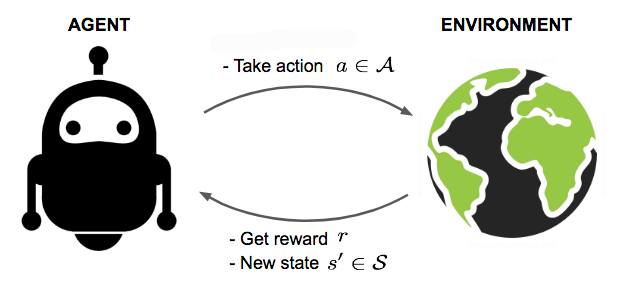
\includegraphics[scale=.5]{RL_illustration.png}
    \caption{Reinforcement Learning}
\end{figure}

As mentioned in the introduction, reinforcement learning is a way of programming agents by reward and
punishment without needing to specify how the task is to be achieved.
As such the primary components of a reinforcement learning problem are an agent which exists in an environment.
From a simplified perspective we can think of the environment as a set of states, actions and rewards.
The objective for the agent is to maximise cumulative reward.
This is done by developing a policy that will dictate which actions should be taken in each state.

\subsection{Explore-Exploit Dilemma}\label{subsec:exploreExploit}
When it comes to reinforcement learning one of the first questions that we have to ask is how we explore
the state space.
An example that is often used to conceptualize this problem is the multi armed bandit problem.
Let's say an agent is in a room with a number of gambling machines.
Each of these machines has an arm that, when pulled will return a reward of 0 or 1 based on some underlying
probability\citep{kaelbling1996reinforcement}.
The agent has a limited number of total pulls.
So the question becomes how do we distributed these pulls in order to maximise return?
Well, first we have to ensure that we explore enough that we find the machine with the best reward probability
and second, we must then exploit this machine to the best of our abilities.

\begin{figure}[ht]
    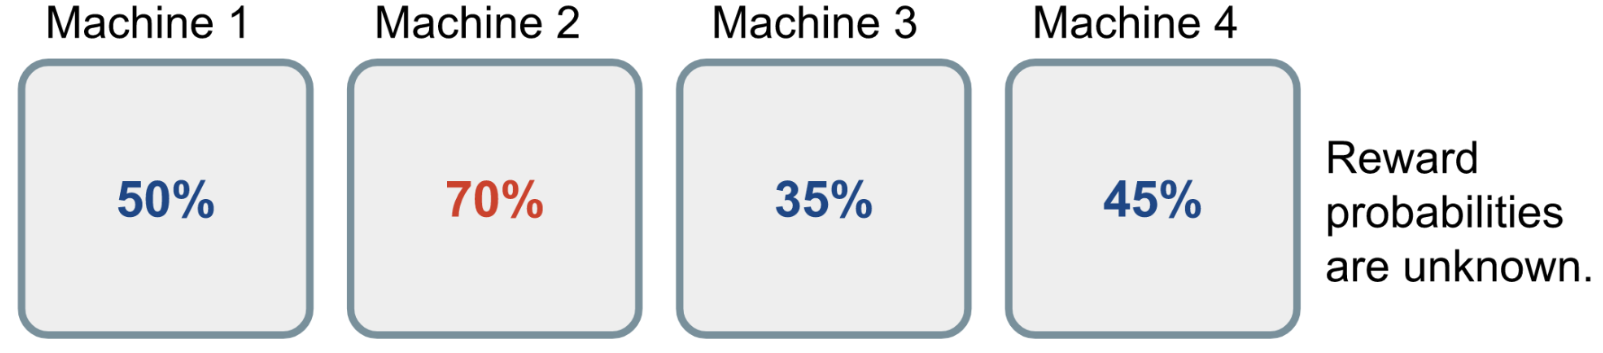
\includegraphics[scale=.25]{bandit.png}
    \caption{Multi Armed Bandit}
\end{figure}

There are a number of approaches that can be taken to solve this problem, we will now briefly discuss two of these
methods.

\subsubsection{$\epsilon$-Greedy Solutions}\label{subsec:eGreedy}
The first approach that we will discuss is the $\epsilon$-greedy strategy.
This approach was first proposed in\citep{watkins1989learning} and is a very simple and widely used method.
The $\epsilon$-greedy strategy involves choosing a random lever some proportion $\epsilon$ of the time, and
choosing the lever that has been established to give the highest reward the rest of the time.

There are a number of variations of this method, the first being the $\epsilon$-first strategy.
With this strategy we take all of our random choices first, allowing us to establish the best bandit,
after which we exploit this bandit.
However, as stated in\citep{vermorel2005multi} this simple approach is sub-optimal because asymptotically,
the constant factor prevents the strategy from getting arbitrarily close to
the optimal lever.

This is where the $\epsilon$-decreasing strategy becomes useful.
Here, the proportion of random lever pulls decreases with time.
Generally if our initial epsilon value is $\epsilon_0$ then our epsilon value at time $t$ will be
$\epsilon_t = \frac{\epsilon_0}{t}$.

\subsubsection{Interval Estimation Strategy}
Another approach that can be used is called the interval estimation strategy.
With this method we initially give an optimistic estimate of the reward to each bandit within a certain
confidence interval.
Then we simply take a greedy approach to our exploration.
Less explored bandits will have a artificially higher reward estimate and thus they will be greedily chosen,
thus allowing us to evaluate each of the bandits.

In the context of reinforcement learning, state space exploration through the $\epsilon$-greedy approach is
generally sufficient.

\subsection{Markov Decision Processes}\label{subsec:mdp}
Reinforcement learning problems are generally modelled according to what is called a markov decision process (MDP).

\begin{itemize}
    \item S - a set of states.
    \item A - a set of actions.
    \item P - a set of state transition probabilities
    \item R - a set of rewards
    \item $\gamma$ - a discount factor
\end{itemize}

\subsection{Policy Evaluation and Policy Improvement}\label{subsec:policyEvalPolicyImp}
As mentioned above the primary focus of reinforcement learning is to find a policy (denoted by $\pi$) that allows
the agent to take actions in states that lead to the maximum possible reward.
There are two primary problems that we must solve in order to do so.

The first is called the prediction problem, also known as policy evaluation.
This involves computing the values of states given some arbitrary policy\citep{sutton1998reinforcement}.
For example a state would have a high value if the reward for reaching that state was high.
A state would also have a high value if we were only one action away, according to the supplied policy,
from a state that renders a high reward.
However a state would have a low value if, according to the policy, there was no path to a state that
would return a positive reward in the foreseeable future.

The second problem is known as the control problem, also known as policy improvement.
This involves changing the policy in order to improve our cumulative reward.
The policy improvement process can only occur when the we have performed policy evaluation.
Let's say, after our evaluation step, we know the value of some state $s$.
Note that this value is calculated with the condition that we take some action $a$ in state $s$.
But, if we take some other action $a'$ would this render a higher value for $s$?
If the answer is yes then we update the policy.

These two operations can be seen as the core of reinforcement learning.
In the next section we will discuss different reinforcement learning methodologies.
Some of the main differences are in how method each approaches the prediction and control problems.

\subsection{Dynamic Programming}\label{subsec:dp}
Dynamic programming (DP) refers to a collection of algorithms that can be used to compute optimal policies given a
perfect model of the environment as a Markov decision process\citep{sutton1998reinforcement}.
Dynamic programming is not widely used in practical reinforcement learning applications due to its assumption
of a perfect MDP and it's high computational requirements.
Despite this it is very important from a theoretical standpoint as it serves as an introduction to a number
of important reinforcement learning concepts.
Furthermore, it provides a basis for many algorithms that are used in practical reinforcement learning applications.

\subsubsection{Policy Evaluation in Dynamic Programming}
When discussion policy evaluation we talk about a state-value function a value function.
This is simply the mapping of states to their corresponding values and is denoted by $v$.

Since the environments's dynamics are completely known we can apply an iterative solution to finding
the value function.
If we consider a series of approximate value functions $v_0, v_1, v_2,..$.
The initial value function, $v_0$ is chosen arbitrarily and each successive generation is obtained by
using the Bellman equation for $v_\pi$ as an update rule\citep{sutton1998reinforcement}:

\begin{align}
    v_{k+1}(s) &= \EX_{\pi}\lbrack R_{t+1} + \gamma v_k(S_{t+1}) | S_t = s \rbrack
\end{align}

In order to produce each successive approximation of $v_{k+1}$ from $v_k$ we apply the operation outlined to each
state $s$.
As shown above our new value for $s$ is based on a combination of the expected immediate rewards($R_{t+1}$),
and the expected values of each of the states that we can transition to($S_{t+1}$) given policy $\pi$.
This operation is applied to each $s$ for each iteration($k$) of the algorithm.
It can be shown that as $k\rightarrow\infty$ $v_k$ will converge to $v_\pi$, the correct value function for policy
$\pi$.
This algorithm is called \textit{iterative policy evaluation}\citep{sutton1998reinforcement}.

\subsubsection{Policy Improvement in Dynamic Programming}
Since we have now determined how good it is to follow $v_\pi$ we can use this information to determine how
we should modify this policy in order to improve it's value.
If we assume that $\pi$ is a deterministic policy then $\pi(s)$ will return some action that we must take.
Now the question becomes what if we take some other action $a \neq \pi(s)$?
Well we must consider whether or not choosing this action, and then continuing to use the existing policy will
improve the value of the policy.
If it does then we will choose this new action.

The logical extension of this approach is to apply it to each state and each possible action.
As such we will select what appears to be the best action at each state.
We can thus denote our new greedy policy $\pi'$ as:
\begin{align}
    \pi'(s) = argmax\EX_{\pi}\lbrack R_{t+1} + \gamma v_k(S_{t+1}) | S_t = s, A_t = a\rbrack
\end{align}
Essentially here we are determining the value of each available action in the current state, using the same operation
as outlined in the policy evaluation phase and choosing.
Then the argmax function will select the action with the highest value.
Finally we assign this action to be the one we will choose in state s, according to the new policy $\pi'$.

\subsection{Monte Carlo}\label{subsec:mc}
In Monte Carlo, unlike dynamic programming, we do not assume complete knowledge of the environment.
Monte Carlo methods require only experience.
We sample sequences of states, actions, and rewards from interaction with the
environment\citep{sutton1998reinforcement}.
Monte carlo evaluation is an episodic process this means that we only update our action values after an episode
has completed.

\subsubsection{Monte Carlo Policy Evaluation}
In Monte Carlo methods we take a fundamentally different approach to policy evaluation.
As mentioned this method is focused on using episodic experience.
As such, in order to evaluate a state we can simply average the rewards returned after visiting that state.
As we observe more returns the average will converge to the actual expected value of the state.

It is worth noting that a state $s$ could be visited more than once in an episode.
As such we can either average the returns following the first visit to $s$ or we could average the returns
after each visit to $s$.
These two methods are called \textit{first-visit} and \textit{every-visit} respectively.

\subsubsection{Monte Carlo Action Values}

\subsubsection{Monte Carlo Policy Improvement}

%Policy evaluation: simply average many returns that start in the state.
%Policy improvement: estimate action values in order to avoid reliance on state transition dynamics.
%(simply choose the best action for the policy in a given state)


\subsection{Temporal Difference Learning (3)}\label{subsec:td}

\section{Game Theory}\label{sec:gameTheory}
After taking a deep dive on reinforcement learning and the papers surrounding RL in texas hold'em it became
clear that a pure reinforcement learning approach would not be feasible.
The main reason for this was the fact that texas hold'em is an imperfect information game.
As outlined by\citep{dahl2001reinforcement}:
\begin{quotation}
Note that the concept of game state values, which is the key to solving perfect information games,
does not apply to imperfect information games, because the players do not know from  which game states they
are choosing.
\end{quotation}
As such it became apparent that some other techniques would have to be incorporated in order to create a competent
texas hold'em agent.
This is when I discovered\citep{heinrich2015fictitious} which utilises a game theoretic model, called
fictitious self-play, as an inspiration for a machine learning based approach to imperfect information games.
In the following section I will discuss elements of game theory that are relevant to this approach.

\subsection{Extensive-form Games}\label{subsec:extensiveForm}
\subsection{Nash Equilibria}\label{subsec:nashEquilibria}
\subsection{Fictitious Play}\label{subsec:fictitiousPlay}

\section{Supervised Learning}\label{sec:supervisedLearning}
Supervised learning involves an agent which observes some example input-output pairs and learns
a function that maps from input to output.\citep{russell2016artificial}.
This learned function can then be used on new input data, that wasn't used to train the agent and the
agent should be able to give an accurate output.
As such this learning task is a generalization problem.
The agent must be able to identify general features of the input data and how they map to the output.
Common examples of

\section{Texas Hold'em}\label{sec:thIntro}
Texas hold'em is one variant of the family of games called poker.
Poker is a group of card games that combine gambling, strategy and skill.
All poker variants have three core similarities.
There is betting involved, there is imperfect information (ie cards remain hidden until the end of a hand)
and the winner is determined by combinations of cards.
We will now discuss texas hold'em poker in more detail.

\subsection{Game Structure}\label{subsec:bettingRounds}
Texas hold'em consists of four betting rounds.
Initially each player is dealt two private cards.
These remain face down and only the person who received these cards may view them.
In the next three rounds five public cards are dealt face up on the table.
The second round of dealing is called the flop, where three cards are dealt.
The third round is called the turn where one additional public card is dealt.
Finally in the fourth round another card is dealt which is called the river.

At each round, after the cards are dealt, the players are given the opportunity to take a number of betting
related actions.
We will discuss the permitted actions in the next section.

In order for players to be incentivized to continue playing in a wider array of situations, blinds are required.
Blinds are a mandatory bet that must be posted by two of the players present at the game.
These two bets are called the big blind and the small blind, the big blind being twice that of the small blind.
As hands are played the big and small blinds are posted by different players in order to distribute the cost fairly.

The big and small blind are the first two bets that contribute to what's called the pot.
The pot is the collection of all of the current chips bet by the players.
When a player wins a hand then what they receive in return is the pot.

The final structural component of the game is player stacks.
Each player will start the game with a certain amount of chips.
If a player wins a pot then all of the chips in the pot are transferred to the winners stack.

\subsection{Actions}\label{subsec:actions}

\subsection{Hand Values}\label{subsec:handValues}

